% 第4章第5节：预算约束下的子集选择（预算约束选择问题；单位成本边际收益法；方法的局限与结果检查）。

\section{预算约束下的子集选择}
\label{sec:graph-budget-selection}

基数约束让每个元素占用一个名额。实际中不同传感器的价格不同，限制的往往是总花费而不是个数。本节说明换成预算约束后，可行集合、选择依据和性能分析各自怎样改变。主线是一种简单可算的逐轮规则，重点放在它的执行过程与失效边界，而不是把上一节的保证直接搬过来。

\subsection{预算约束选择问题}
\label{sec:graph-setfn-budget-problem}

给每个元素$v\in V$指定成本$c_v$，再给定总预算$B\geq0$。要求的是
\begin{equation}
  \max_{S\subseteq V}\ F(S)\qquad\text{满足}\quad\sum_{v\in S}c_v\leq B.
  \label{eq:graph-setfn-budget-problem}
\end{equation}
满足成本条件的子集称为预算可行的，这一条件称为\term{预算约束}（budget constraint）。目标函数$F$与上一节相同，改变的只是允许的子集。所有成本都取$1$、预算取$k$时，预算约束就是基数约束，所以本节的问题是上一节的推广。

成本可能为零的元素需要先单独处理。零成本元素不占预算，若$F$单调，把它们全部加入不会降低目标，可以在开始时一次放进集合；若$F$不单调，它们是否值得加入要看增益的正负。以下设所有成本为正。另外，成本超过$B$的元素不可能出现在任何可行集合中，可以预先删去。

\paragraph{两种约束下的可行集合}
在传感器实例中取成本$c_a=4$、$c_b=3$、$c_c=4$、$c_d=1$，预算$B=7$。预算可行的子集共有$10$个：空集、四个单元素集，以及$\{a,b\}$（成本$7$）、$\{a,d\}$（$5$）、$\{b,c\}$（$7$）、$\{b,d\}$（$4$）、$\{c,d\}$（$5$）；三元及以上的子集成本都超过$7$。枚举得最优集合为$\{b,c\}$，覆盖$16$格。与$k=2$的基数约束相比，$\{a,c\}$成本为$8$，现在不可行了；而$\{a,b\}$在两种约束下都可行。选择的个数不再直接决定资源消耗，每次加入元素前都要检查剩余预算。

\subsection{单位成本边际收益法}
\label{sec:graph-setfn-ratio-greedy}

把上一节的贪心原样搬过来，就是每轮在付得起的元素里选增益最大的。这样做会偏爱昂贵的元素：一个元素增益大，可能只是因为它贵。更合理的比较是每单位成本带来多少增益。

\begin{algorithm}[预算约束下的单位成本贪心]
\label{alg:graph-setfn-ratio-greedy}
输入：有限底集$V$（元素已编号），正成本$c_v$，预算$B\geq0$，单调非减集合函数$F$的求值规则。输出：预算可行的集合。状态：已选集合$S$，剩余预算$R=B-\sum_{v\in S}c_v$，本轮候选元素的增益。
\begin{enumerate}
  \item 令$S=\varnothing$，$R=B$。
  \item 记候选集合$Q=\{v\in V\setminus S:c_v\leq R\}$。若$Q$为空，停止。
  \item 对每个$v\in Q$计算$\Delta(v\mid S)$。若这些增益全为零，停止；否则取比值$\Delta(v\mid S)/c_v$最大的$v$，比值相同时取编号最小者。
  \item 令$S\leftarrow S\cup\{v\}$，$R\leftarrow R-c_v$，回到第2步。
\end{enumerate}
\end{algorithm}

每轮至少加入一个元素，所以算法至多执行$n$轮，求值次数不超过$n+(n-1)+\cdots+1=n(n+1)/2$。停止时有两种原因：没有付得起的元素，或者付得起的元素都不再增加覆盖。

\paragraph{两种规则的对照}
图~\ref{fig:graph-setfn-budget-rule-comparison}在$B=7$的实例上比较“总增益最大”与“单位成本增益最大”两种规则。按总增益，第$1$轮选$a$（增益$10$），剩余预算$3$；第$2$轮付得起的有$b$（增益$2$）和$d$（增益$1$），$c$的成本$4$超出剩余预算，选$b$，剩余预算$0$，停止，覆盖$12$格。按单位成本，第$1$轮的比值为$a:10/4=2.5$，$b:8/3\approx2.67$，$c:8/4=2$，$d:1/1=1$，选$b$，剩余预算$4$；第$2$轮相对于$\{b\}$，$a$的增益为$4$（第$5$、$6$列），比值$1$，$c$的增益为$8$，比值$2$，$d$的增益为$0$，选$c$，剩余预算$0$，停止，覆盖$16$格，恰为枚举最优值。

\begin{figure}[!htb]
  \centering
  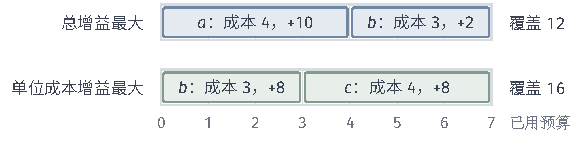
\includegraphics[width=98.538mm]{figures/01-basic-mathematics/04-graphs/tikz/c4-budget-rule-comparison/figure.pdf}
  \caption{预算$B=7$下两种逐轮规则的选择结果（成本$c_a=4$、$c_b=3$、$c_c=4$、$c_d=1$）。每条横条代表$7$个单位的预算，色块的宽度是所选元素的成本，块内写出选择时的增益。按总增益先选昂贵的$a$，剩余预算只够再选增益$2$的$b$，覆盖$12$格；按单位成本先选$b$，再选$c$，覆盖$16$格。}
  \label{fig:graph-setfn-budget-rule-comparison}
\end{figure}

\paragraph{与最佳单元素比较}
单位成本规则也有自己的偏差：它可能先选几个便宜的小元素，把预算切碎，使一个昂贵但价值很高的元素再也放不进去。一种简单的补救是在算法结束后，再计算每个可行单元素的值$F(\{v\})$（$c_v\leq B$），输出$S$与最佳单元素中函数值较大的一个。这只需另外$n$次求值。在$B=7$的实例中，最佳单元素是$\{a\}$，覆盖$10$格，小于$16$，输出仍是$\{b,c\}$。这一检查只是一个具体策略；本节没有给出它的分析，因此不附加一般的近似比例。

\subsection{方法的局限与结果检查}
\label{sec:graph-setfn-budget-limits}

单位成本规则在上面的实例中表现很好，但下面的例子说明它本身没有任何固定比例的保证。

\begin{example}[比值规则的失效]
\label{ex:graph-setfn-ratio-failure}
底集$\{u,w\}$，预算$B=100$。$u$的成本为$1$、价值为$2$，$w$的成本为$100$、价值为$100$，目标取模函数$F(S)=\sum_{v\in S}(\text{价值})$。它单调，也是次模的。

比值规则第$1$轮比较$2/1=2$与$100/100=1$，选$u$；剩余预算$99<100$，$w$付不起，算法停止，得$F(\{u\})=2$。最优选择是$\{w\}$，$F=100$。见图~\ref{fig:graph-setfn-budget-ratio-failure}。把$w$的成本、价值与预算同时换成任意大的$M$，比值规则仍先选$u$，得到$2$而最优值为$M$，比例$2/M$可以任意小。
\end{example}

\begin{figure}[!htb]
  \centering
  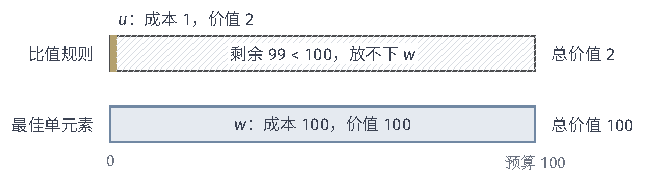
\includegraphics[width=109.146mm]{figures/01-basic-mathematics/04-graphs/tikz/c4-budget-ratio-failure/figure.pdf}
  \caption{比值规则的失效例。横条长度代表预算$100$。上行：比值规则先选单位价值较高的$u$（黄色，成本$1$，为便于观察略加宽），剩余$99$个单位（斜线）放不下成本$100$的$w$，总价值$2$。下行：最佳单元素$w$恰好用满预算，总价值$100$。}
  \label{fig:graph-setfn-budget-ratio-failure}
\end{figure}

这个例子的目标是模函数，从而单调且次模，可见即使目标满足上一节定理的全部函数条件，原始比值规则也不能继承那里的保证：预算约束改变了可行集合的结构，证明中“最优集合至多$k$个元素”这一步不再有对应物。上一小节的最佳单元素比较能修复这个例子，因为它会发现$\{w\}$；但修复一个例子不构成一般保证。具有严格保证的预算选择算法需要另外的枚举或修正机制，并要给出相应的证明，本书不展开，也不应把它们与这里的简单规则混为一谈。

\paragraph{结果检查}
小实例可以直接枚举全部预算可行子集，核对三件事：输出集合的总成本不超过预算，输出的函数值计算无误，以及它与枚举最优值的差距。上面$B=7$的实例只有$10$个可行子集，比值规则的结果$\{b,c\}$与枚举最优一致，总增益规则的结果$\{a,b\}$差$4$格。大实例无法枚举时，至少应报告所用预算与剩余预算、最终目标值、最佳单元素的值，以及总求值次数和每次求值的代价。最佳单元素给出一个必须超过的基准；若逐轮规则的结果不如它，往往就是出现了示例~\ref{ex:graph-setfn-ratio-failure}那样预算被小元素切碎的情形。
